\documentclass[a4paper,5p]{elsarticle}

\usepackage[utf8]{inputenc}
\usepackage[T5]{fontenc}
\usepackage{amsmath}
\usepackage{amssymb}
\usepackage{booktabs}
\usepackage{tabularx}
\usepackage{array}
\usepackage{graphicx}
\usepackage{xcolor}
\usepackage{dblfloatfix}
\usepackage{microtype}
\usepackage{xurl}
\usepackage[hidelinks]{hyperref}

\journal{Image and Vision Computing}

\newcommand{\method}{PACE-Seg}
\newcommand{\miou}{mIoU}
\newcommand{\etal}{et al.}
\setlength{\emergencystretch}{2em}
\hfuzz=3pt

\begin{document}

\begin{frontmatter}

\title{PACE-Seg: When Does Input-Adaptive Semantic Segmentation Pay Off on Edge Accelerators?}

% TODO(author): confirm author list/order, full affiliation postal addresses, and corresponding e-mail.
\author[aff1]{D\~ung Nguy\~{\^e}n\corref{cor1}}
\ead{[CORRESPONDING-AUTHOR-EMAIL]}
\cortext[cor1]{Corresponding author.}
\affiliation[aff1]{organization={[DEPARTMENT, INSTITUTION]},
            addressline={[STREET ADDRESS]},
            city={[CITY]},
            postcode={[POSTCODE]},
            country={[COUNTRY]}}

\begin{abstract}
Input-adaptive inference promises to spend computation only where an image needs it, but on an edge accelerator an adaptive pipeline also pays for probing, deciding, and switching engines. We measure when this trade-off favours adaptivity, using \method{}, an elastic semantic-segmentation model whose four capacities are exported as separately compiled static TensorRT and Hailo-8 engines, and a family of budget-aware routers driven by one entropy probe. Candidate latency is measured on four edge devices, and complete routes and static deployments are timed in one harness on the two primary backends, with Cityscapes and four ACDC conditions. The capacities span $110.2\times$ in FLOPs but only $12.3$--$18.1\times$ in measured mean latency, so a FLOPs-proportional proxy does not reproduce measured budget choices. Shared elastic training costs the largest capacity 0.9 \miou{} points on Cityscapes and 1.6--2.8 points on ACDC relative to the same architecture trained alone. Among routers, the hard measured budget and operating-point tuning matter: routing under a hard budget outperforms rank escalation by 2.87 points on fair cells (95\% CI 2.52--3.26), whereas candidate-specific calibration shows no detectable gain over a tuned three-threshold scalar router ($-0.03$ points; the 95\% CI, $-0.11$ to $0.09$, excludes gains larger than 0.09 points). When each static model is charged its own measured latency and both are compared at budgets where a route is feasible, static deployment outperforms routing by 3.0 points on a TensorRT GPU and 8.2 points on a Hailo-8, because probing and switching add 0.7--2.7~ms and 38--47~ms per frame; at 12.5\% and 37.5\% of the evaluated budget cells, only the static model fits at all. A counterfactual analysis that scales the measured overhead shows that routing would pay off only under mean-cost budgets and only if this overhead fell below about 1.3 and 4.3~ms; adaptive segmentation studies should therefore report a static baseline timed in the same harness.
\end{abstract}

\begin{keyword}
semantic segmentation \sep dynamic inference \sep elastic neural networks \sep edge acceleration \sep hardware-aware deployment \sep latency measurement
\end{keyword}

\end{frontmatter}

%======================================================================
\section{Introduction}
\label{sec:introduction}

A vehicle or mobile robot that segments its surroundings on an embedded accelerator must return a label map within a per-frame latency budget set by its control loop. Two things make that budget hard to honour with a single network. First, visual difficulty varies from frame to frame: the same 19 semantic classes appear in clear daylight, fog, rain, snow, and at night (Fig.~\ref{fig:teaser}a), and a model that is sufficient for a clear frame can fail on a dark one. Second, the cost of a given network depends on the accelerator that runs it: a capacity that fits the budget on one device may not fit on another (Fig.~\ref{fig:teaser}b). A model chosen offline must therefore be sized for the hardest condition on the slowest device, which wastes capacity on easy frames, or it must accept budget violations.

Elastic networks offer several capacities from one set of trained weights~\cite{yu2019usnet,cai2020ofa}, but they leave open which capacity a given image warrants under a given device budget. Answering that question at run time usually involves two shortcuts. Compute counts such as FLOPs stand in for device latency, and a single confidence score stands in for difficulty without asking which alternative capacity would actually reduce the error. Both shortcuts can be replaced by a measured or calibrated quantity, but a third cost is usually left out: the adaptive pipeline itself must probe, decide, and switch engines, which a static deployment never does (Fig.~\ref{fig:teaser}c). This paper asks when, once all three costs are measured on real accelerators, input-adaptive segmentation actually beats deploying one static model.

We study this question with \method{}, a test bed in which every ingredient can be switched off and every cost is measured. A compiler-safe elastic model provides four capacities, tiny to large, each exported as an independent static graph. Each target device contributes a measured table of complete inference-route costs, including the probe and dispatch overhead, and of static deployment costs, timed in the same harness. For each image, the tiny candidate produces a segmentation and a mean-entropy score; a family of routers maps that score to a capacity under the budget, from rank escalation through a tuned threshold rule to candidate-specific calibrated risk (Fig.~\ref{fig:condition-probe-routes}).

We evaluate the design through three research questions on Cityscapes, four ACDC conditions, and four edge devices (Table~\ref{tab:study-setting}). RQ1 asks whether a FLOPs-proportional proxy reproduces measured hardware feasibility; it does not, because a $110.2\times$ compute range becomes only a $12.3$--$18.1\times$ latency range. RQ2 asks whether shared elastic training degrades quality; it does, moderately: the largest capacity is 0.9 \miou{} points below the same architecture trained alone on Cityscapes and 1.6--2.8 points below on the ACDC conditions. RQ3 asks which routing ingredients matter and whether routing beats static deployment. With measured route costs on a TensorRT GPU and a Hailo-8 accelerator, the hard budget and fit-half operating-point tuning account for the gain over rank escalation, and candidate-specific calibration shows no detectable gain over a tuned three-threshold scalar router. Against static deployment charged its own measured latency, routing loses on both accelerators, and a counterfactual break-even analysis quantifies how small the routing overhead would have to become.

The contributions are:
\begin{enumerate}
    \item a measurement methodology that times separately compiled static candidates, complete inference routes, and static deployments with one harness and one timer boundary on a TensorRT GPU and a Hailo-8, and shows that a FLOPs-proportional proxy misstates feasibility;
    \item a same-harness comparison of adaptive routing with static deployment and a break-even analysis of the routing overhead, which identify the conditions under which adaptive segmentation pays off on these accelerators;
    \item an ablation of budget-aware routing that separates the hard budget, operating-point tuning, and candidate-specific calibration, with image-level and nested bootstrap intervals, showing no detectable benefit of candidate-specific calibration over tuned scalar thresholds with a single probe;
    \item compiled-engine accuracy for TensorRT FP16 and Hailo-8 INT8 and an on-device replay that confirm the conclusions with the deployed engines.
\end{enumerate}

Section~\ref{sec:related} positions the work. Section~\ref{sec:method} follows one image through \method{}, Section~\ref{sec:protocol} describes the data, hardware, and evaluation protocol, and Section~\ref{sec:results} answers RQ1--RQ3. Section~\ref{sec:discussion} discusses when routing pays off, what drives the gain among routers, and what the study does not establish.

\begin{figure*}[!t]
\centering
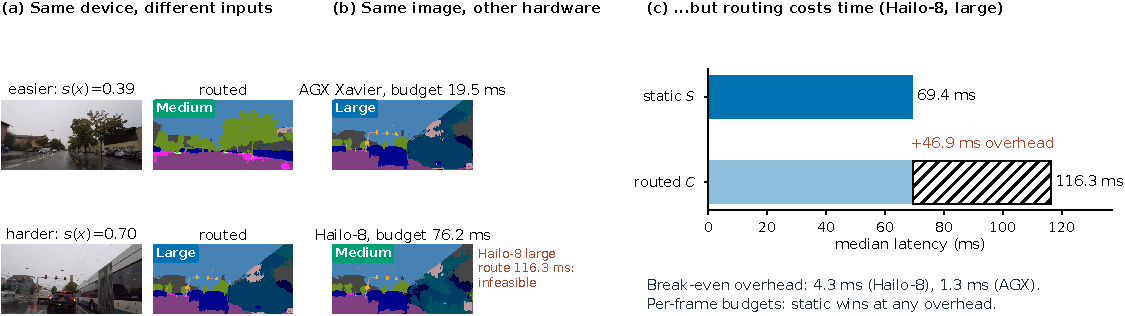
\includegraphics[width=\textwidth]{figures/fig1_teaser_v20.pdf}
\caption{Adaptive capacity selection on an edge accelerator, and its price. (a) On one device (AGX Xavier, budget of the large route), an easier and a harder held-out ACDC rain image receive different capacities from policy D. (b) The same harder image receives large on AGX Xavier but medium on the Hailo-8, where the large route exceeds the budget. (c) On Hailo-8 the route to large costs 46.9~ms more than deploying large statically, because the probe, decision, and engine switch must run first; overheads of this size erase the adaptive gain (Section~\ref{sec:rq3}). Images are the frozen `easier' and `harder' rain selections of Section~\ref{sec:rq3}; decisions are those of Run A.}
\label{fig:teaser}
\end{figure*}

\begin{table}[!t]
\centering
\caption{Study setting at a glance. Candidate-only latency is measured on four devices; complete routed latency, including probing and decision overhead, and static latency are measured on the two primary accelerator backends.}
\label{tab:study-setting}
\small
\begin{tabularx}{\columnwidth}{@{}>{\bfseries}lX@{}}
\toprule
Component & Evaluated setting \\
\midrule
Visual domains & Cityscapes clean and ACDC fog, night, rain, and snow \\
Prediction task & Semantic segmentation over the 19 Cityscapes train classes \\
Elastic choices & Tiny, small, medium, and large static capacities \\
Candidate-cost devices & Hailo-8, Xavier NX, AGX Xavier, Orin Nano \\
Complete-route backends & Hailo-8 and AGX Xavier (TensorRT) \\
Router protocol & Alternating fit/held-out validation halves; three training seeds \\
\bottomrule
\end{tabularx}
\end{table}

%======================================================================
\section{Related work}
\label{sec:related}

\subsection{Efficient semantic segmentation}

Fully convolutional networks established dense end-to-end prediction~\cite{long2015fcn}, and pyramid pooling and atrous encoder--decoders raised accuracy at substantial computational cost~\cite{zhao2017pspnet,chen2018deeplabv3plus}. Real-time designs reduce that cost in several ways. ENet and ERFNet use early downsampling and factorized convolutions~\cite{paszke2016enet,romera2018erfnet}, ICNet cascades low- and high-resolution branches~\cite{zhao2018icnet}, and Fast-SCNN shares a learning-to-downsample module between a global feature extractor and a high-resolution path~\cite{poudel2019fastscnn}. Fast-SCNN serves as our matched-capacity comparator because it occupies a similar sub-million-parameter regime with the depthwise-separable operators that also underlie mobile classification networks~\cite{sandler2018mobilenetv2,howard2019mobilenetv3}.

Current real-time models are dominated by two-branch and multi-resolution designs. BiSeNet and BiSeNetV2 separate spatial detail from semantic context~\cite{yu2018bisenet,yu2021bisenetv2}, STDC replaces the extra spatial path with detail-guided training~\cite{fan2021stdc}, DDRNet maintains bilateral dual-resolution fusion~\cite{pan2023ddrnet}, and PIDNet adds a boundary branch inspired by PID control~\cite{xu2023pidnet}. SegFormer and OffSeg improve the accuracy--efficiency frontier through efficient attention and offset-based feature alignment~\cite{xie2021segformer,zhang2025offseg}. Despite their different mechanisms, these models share one deployment assumption: after compilation, every image passes through the same operating point. \method{} is complementary to this line. Any family of compilable candidates could replace its elastic encoder--decoder; we keep one family fixed so that routing effects are not confounded with architectural differences.

\subsection{Elastic and input-adaptive networks}

Slimmable networks train shared weights at several preset widths with switchable batch normalization, and US-Net extends this to arbitrary widths with the sandwich rule and in-place distillation~\cite{yu2019slimmable,yu2019usnet}. Once-for-All trains a broader depth--width--resolution--kernel space and extracts a specialized subnetwork for each target under a latency predictor~\cite{cai2020ofa}. SlimSeg brings slimmable training to segmentation with stepwise distillation~\cite{xue2022slimseg}, and recent width-adaptive ConvNeXt models target deployment of one network across devices with different resource limits~\cite{haberer2026slimmableconvnext}. \method{} adopts the sandwich rule and in-place distillation, but freezes each capacity into a separate static graph instead of switching widths inside one dynamic model, which keeps the engines compatible with accelerators such as Hailo-8 that do not execute data-dependent control flow.

A related line adapts computation to each input. Early-exit classifiers such as BranchyNet and MSDNet stop at an intermediate predictor once confidence is sufficient~\cite{teerapittayanon2016branchynet,huang2018msdnet}, and SkipNet and BlockDrop learn per-input layer or block execution~\cite{wang2018skipnet,wu2018blockdrop}; Han~\etal{} survey these sample-, spatial-, and temporal-wise variants~\cite{han2022dynamic}. For dense prediction, Dynamic Routing selects scale-transform paths with learned gates~\cite{li2020dynamic}, Anytime Dense Prediction refines its output through confidence-adaptive exits~\cite{liu2022anytime}, and MESS chooses among the exits of a multi-exit segmentation network~\cite{kouris2022mess}. Most of these methods express cost through FLOPs or a soft training penalty and execute their adaptivity inside one graph. \method{} moves the decision outside the graph and constrains it by measured latency, at the price of coarser granularity: it chooses among four engines rather than among layers or exits.

\subsection{Hardware-aware design and latency modelling}

MnasNet made measured on-device latency a search objective~\cite{tan2019mnasnet}, and ProxylessNAS and FBNet searched directly on target hardware or through latency lookup tables~\cite{cai2019proxylessnas,wu2019fbnet}. FasterSeg, AutoSegEdge, multi-objective edge NAS, RealtimeSeg, and HARD bring platform cost into segmentation architecture design~\cite{chen2020fasterseg,dou2023autosegedge,dou2024multiobjective,li2023realtimeseg,kwon2024hard}. HW-NAS-Bench documented that FLOPs and measured latency diverge across devices~\cite{li2021hwnasbench}, and nn-Meter predicts kernel-level latency for unseen models~\cite{zhang2021nnmeter}. All of these use hardware cost to choose one architecture before deployment. \method{} uses cost at run time to restrict a fixed candidate set per device; because the set is small, every complete route can be measured directly and no latency predictor is needed. RQ1 accordingly evaluates only a proportional FLOPs proxy and makes no claim about learned predictors.

\subsection{Uncertainty and calibration under adverse conditions}

Monte Carlo dropout, deep ensembles, and aleatoric--epistemic decompositions estimate predictive uncertainty~\cite{gal2016dropout,lakshminarayanan2017ensembles,kendall2017uncertainties}, but require multiple passes or extra heads that are costly on edge accelerators. Modern networks are often miscalibrated~\cite{guo2017calibration}, and monotone post-hoc mappings such as histogram binning and isotonic regression are standard corrections~\cite{zadrozny2002isotonic}. Selective prediction asks whether a score ranks errors correctly and summarizes this with risk--coverage curves and AURC~\cite{geifman2017selective}; conformal risk control adds distribution-free guarantees under exchangeability~\cite{angelopoulos2024crc}. In segmentation, calibration degrades under domain shift and differs across model capacities~\cite{wang2023calibrating,dejorge2023reliability}. Foggy Cityscapes and Dark Zurich target fog and night~\cite{sakaridis2018foggy,sakaridis2019darkzurich}, and ACDC provides real fog, night, rain, and snow images with Cityscapes-compatible labels~\cite{sakaridis2021acdc}. \method{} uses a single-pass entropy score and a separate binned monotone calibrator per candidate; its estimates support risk-aware selection but provide no formal risk guarantee.

\subsection{Positioning}

Table~\ref{tab:related-positioning} compares the closest methods by how they construct candidates, when they select, and how they represent cost and risk. Most input-adaptive methods report savings in FLOPs or against static baselines with idealized costs. What the present experiments establish is narrower and deployment-oriented: separately compiled static candidates, measured complete inference routes on TensorRT and Hailo-8, a static comparison timed in the same harness, compiled-engine validation, and the break-even overhead at which adaptivity would pay off. Candidate-specific calibrated risk is one of the evaluated routers, not a component the results show to be necessary.

\begin{table*}[!t]
\centering
\caption{Mechanism-level positioning relative to representative primary work. Entries summarize the stated operating mechanism rather than rank methods or claim exhaustive coverage. ``Complete route'' includes the probe, risk computation, policy decision, backend dispatch or activation, and any additional candidate inference.}
\label{tab:related-positioning}
\footnotesize
\setlength{\tabcolsep}{3pt}
\begin{tabular*}{\textwidth}{@{\extracolsep{\fill}}lllllll@{}}
\toprule
Method & Candidates & Selection & Cost model & Risk signal & Budget & Deployed form \\
\midrule
Once-for-All~\cite{cai2020ofa} & Elastic subnetworks & Design time & Latency predictor & None & Design constraint & Static subnet \\
SlimSeg~\cite{xue2022slimseg} & Slimmable widths & Configured & Efficiency setting & None & None & Static width \\
MESS~\cite{kouris2022mess} & Multi-exit network & Per image & Exit latency & Exit confidence & Soft, per exit & Multi-exit graph \\
Dynamic Routing~\cite{li2020dynamic} & Multi-scale paths & Per image & Compute penalty & Learned gates & Soft penalty & Dynamic graph \\
AutoSegEdge~\cite{dou2023autosegedge} & Searched network & Design time & FLOPs + latency & None & Search constraint & Static network \\
\method{} & Four capacities & Per image & Measured route & Entropy probe & Hard, measured & Static engines \\
\bottomrule
\end{tabular*}
\end{table*}

%======================================================================
\section{PACE-Seg}
\label{sec:method}

Figure~\ref{fig:condition-probe-routes} summarizes how \method{} processes one image. Two quantities are computed independently. Visual risk is estimated per image from a cheap probe, and hardware cost is measured once per device. They meet only in the policy, which selects one static engine. This section describes the candidate family that the policy chooses from (Section~\ref{sec:elastic}), the two estimated quantities (Sections~\ref{sec:measured-cost} and~\ref{sec:calibration}), the policy itself (Section~\ref{sec:policy}), and a complete worked decision (Section~\ref{sec:example}).

\begin{figure*}[!t]
\centering
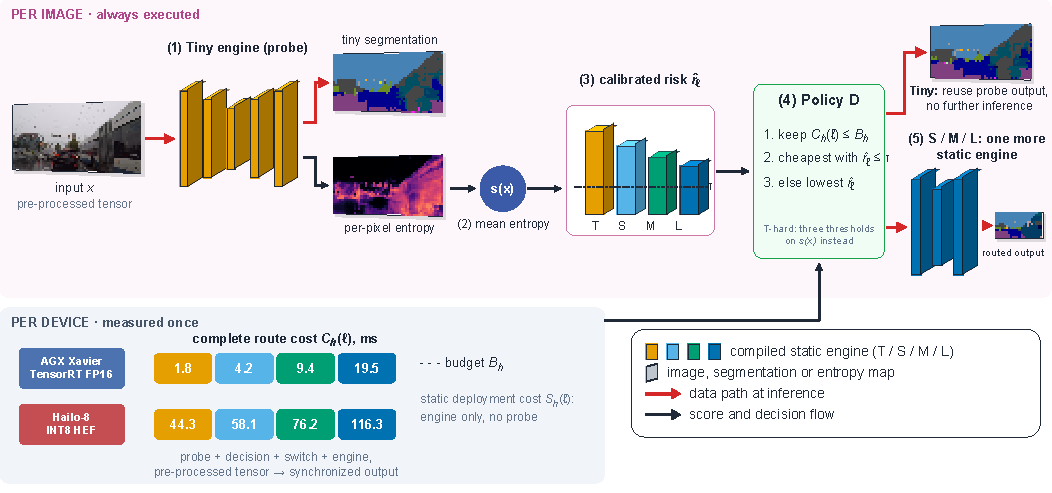
\includegraphics[width=\textwidth]{figures/fig2_pipeline_v20.pdf}
\caption{\method{} inference. The tiny probe always runs first: it produces a segmentation and its mean entropy $s(x)$, which candidate-specific calibrators $g_\ell$ map to expected errors $\hat r_\ell$ (top lane). Hardware cost is measured once per device as the complete inference-route cost $C_h(\ell)$, from a preprocessed host tensor to synchronized output, together with the budget $B_h$ (bottom lane). If the policy selects tiny, the probe output is returned with no further inference; otherwise one additional static engine runs after the probe. A static deployment runs only its own engine and pays $S_h(\ell)$. Fig.~\ref{fig:input-output-pipeline} gives a numerical instance.}
\label{fig:condition-probe-routes}
\end{figure*}

\subsection{Compiler-safe elastic candidate family}
\label{sec:elastic}

The four candidates, tiny, small, medium, and large, are extracted from one shared encoder--decoder by jointly varying three axes: width multiplier (0.25, 0.50, 0.75, 1.00), repeated-block depth (2, 3, 4, 6), and input resolution ($384\times192$, $512\times256$, $768\times384$, $1024\times512$, width$\times$height, matching the 2:1 aspect of Cityscapes and ACDC). The candidates share convolutional weights through active-channel slicing, while each keeps its own batch-normalization statistics, following slimmable training practice~\cite{yu2019slimmable}; activation statistics of a 0.25-width, $384\times192$ path differ substantially from those of the full-width, $1024\times512$ path. The network uses only standard operators and fixed-factor resizing, so each candidate exports as a fixed-shape ONNX graph and compiles to a static TensorRT or Hailo-8 engine (Fig.~\ref{fig:candidate-family}). Routing therefore chooses an engine before execution and never introduces data-dependent control flow into a graph.

\begin{figure*}[!t]
\centering
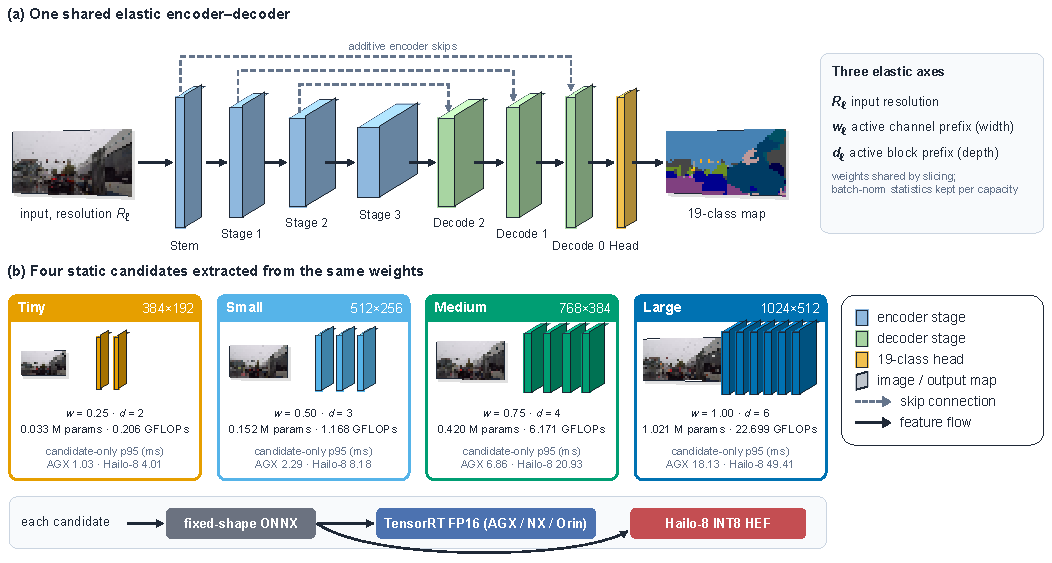
\includegraphics[width=\textwidth]{figures/fig2_architecture_v20.pdf}
\caption{Elastic architecture and static extraction. (a) One shared encoder--decoder: a stem, three downsampling depthwise-separable encoder stages, three top-down decoder stages with additive encoder skips, and a 19-class head; input resolution $R_\ell$, active channel prefix $w_\ell$, and active block prefix $d_\ell$ define elasticity. (b) Tiny through large freeze those axes into four static graphs, exported through fixed-shape ONNX to TensorRT GPU or Hailo-8. Card values are input size (width$\times$height), parameters, GFLOPs, and candidate-only p95 latency on AGX Xavier and Hailo-8; complete route costs are measured separately (Table~\ref{tab:routes}).}
\label{fig:candidate-family}
\end{figure*}

All candidates are trained together with the sandwich rule~\cite{yu2019usnet}. Each step samples the smallest level, the largest level, and one randomly chosen intermediate level; every sampled level receives the batch resized to its own resolution. Each level is supervised with a boundary-aware cross-entropy, $\mathcal{L}_{\mathrm{seg}}=\mathrm{CE}+\lambda_b\,\mathrm{CE}_w$, where $\mathrm{CE}_w$ reweights label-boundary pixels by three and $\lambda_b=1$. Every level except the largest additionally receives in-place distillation~\cite{hinton2015distilling} from the detached, resized logits of the largest level, $\alpha\,T^2\,\mathrm{KL}(p_{\mathrm{large}}^{T}\,\|\,p_\ell^{T})$ over non-ignore pixels, with $\alpha=0.5$ and $T=1$; the step loss sums all sampled levels. Training runs for 100,000 steps with batch size 8 and AdamW (initial learning rate $3\times10^{-4}$, weight decay $10^{-4}$), 500 warm-up steps followed by cosine decay, gradient clipping at 5.0, and FP16 mixed precision. The Cityscapes and ACDC training sets are concatenated without reweighting, and augmentation applies random scaling in $[0.75,1.25]$, padding and cropping, horizontal flipping with probability 0.5, and colour jitter of 0.3 in brightness, contrast, and saturation.

\subsection{Measured route cost}
\label{sec:measured-cost}

For a target device $h$ and candidate $\ell$, the policy uses the measured complete inference-route cost $C_h(\ell)$, the time from handing a preprocessed host tensor to the runtime until the selected candidate's output is synchronized; image decoding, resizing, and normalization are excluded. A route always begins with the tiny probe, so $C_h(\ell)$ includes tiny inference, entropy, calibrator and policy evaluation, backend dispatch or activation, and, unless tiny itself is selected, inference of the chosen candidate. When tiny is selected, its probe prediction is returned directly. Because cost enters only after training, deploying to a new device requires compiling the four graphs and measuring their four routes, with no change to weights or calibrators. Section~\ref{sec:rq1} shows why this measurement cannot be replaced by FLOPs. For comparison with static deployment we also measure the static cost $S_h(\ell)$ of running candidate $\ell$ alone, without the probe, in the same harness.

\subsection{Candidate-specific visual risk}
\label{sec:calibration}

Let the tiny candidate produce logits $z(x)$ for image $x$, with softmax probabilities $p_{u,c}$ at pixel $u$ for class $c$. The probe score is mean pixel entropy,
\begin{equation}
s(x)=\frac{1}{|\Omega|}\sum_{u\in\Omega}-\sum_{c=1}^{C}p_{u,c}\log\max(p_{u,c},10^{-12}),
\label{eq:entropy}
\end{equation}
over all output pixels $\Omega$, with $C=19$. For each candidate $\ell$, a monotone calibrator $g_\ell$ maps the shared score to that candidate's expected per-image pixel error,
\begin{equation}
\widehat{r}_\ell(x)=g_\ell(s(x)).
\label{eq:risk}
\end{equation}
Each $g_\ell$ is fitted on the fit half of the data only: fit-half scores are divided into ten equal-count bins, the mean observed error of candidate $\ell$ is computed in each bin over non-ignore pixels, and a cumulative-maximum pass enforces monotonicity. The primary configuration fits one calibrator set per visual condition; a pooled variant fits one set on all five fit halves and removes the need to know the condition at run time.

Three properties motivate this design. The probe costs no extra network, because the tiny engine is itself a deployable route and its entropy needs only one softmax and one reduction, a cost already contained in every measured route. Multi-pass estimators such as Monte Carlo dropout or ensembles~\cite{gal2016dropout,lakshminarayanan2017ensembles} would multiply that cost. A scalar score does not directly provide candidate-specific error estimates; the calibrators convert it into an interpretable risk vector, and Section~\ref{sec:rq3} tests whether this additional structure improves routing over tuned scalar thresholds. Finally, binned monotone calibration~\cite{zadrozny2002isotonic} has few parameters per candidate and cannot reverse the ordering implied by the score, which limits overfitting on fit halves of 50--250 images per split.

\subsection{Hardware-cost-conditioned policy}
\label{sec:policy}

Given the risk vector $\widehat{r}_\ell(x)$, the cost table $C_h(\ell)$, a budget $B_h$, and a risk target $\tau$, policy D first forms the feasible set
\begin{equation}
\mathcal{S}_h=\{\ell : C_h(\ell)\leq B_h\}.
\label{eq:feasible}
\end{equation}
If some feasible candidate satisfies $\widehat{r}_\ell(x)\leq\tau$, D selects the cheapest such candidate; otherwise it selects the feasible candidate with the lowest predicted error, breaking ties by cost. If $\mathcal{S}_h$ is empty, that is, $B_h<C_h(\mathrm{tiny})$, D returns the tiny probe output, the cheapest possible route. With four candidates the decision costs four table lookups and four comparisons, independent of image resolution. A new device changes only $C_h$; a new visual domain changes only $g_\ell$.

The main comparator, policy A, uses the same calibrated probe score $\widehat{r}_{\mathrm{tiny}}(x)$ but escalates by latency rank: it selects the cheapest candidate if the score is at most $\tau$ and otherwise the candidate at latency rank $\lfloor \widehat{r}_{\mathrm{tiny}}(x)/\tau\rfloor$, counting the cheapest as rank 0 and capping at large. A has neither candidate-specific risk nor a hard budget. To separate these two ingredients, A-hard applies D's feasibility mask to A: whenever A's choice exceeds $B_h$, it is replaced by the most expensive feasible candidate. A-hard therefore has a hard budget but no candidate-specific risk. T-hard asks whether candidate-specific calibration is needed at all: it applies three monotone thresholds directly to $s(x)$, fitted on the fit half to maximize fit-half \miou{} under the budget, with the same feasibility mask. Table~\ref{tab:policy-summary} lists all evaluated policies and the information each may access. Two static references run one capacity without the probe: the best feasible static candidate, the largest whose cost fits the budget, and, for mean-cost budgets, a random mixture of two adjacent static candidates. A per-image ground-truth pixel-error oracle, which selects for each image the feasible candidate with the lowest observed pixel error, serves as a non-deployable reference; because it optimizes per-image pixel error rather than dataset-level \miou{}, it is not a formal upper bound.

\begin{table*}[!t]
\centering
\caption{Routing policies and information access. ``Per condition'' means that the deployment domain is configured before inference; pooled D removes that requirement. The oracle uses held-out ground-truth pixel error and is not deployable.}
\label{tab:policy-summary}
\small
\resizebox{\textwidth}{!}{%
\begin{tabular}{@{}lcccc l@{}}
\toprule
Policy & Candidate risk & Hard budget & Calibrator & Deployable & Purpose \\
\midrule
Best feasible static & No & Yes & None & Yes & Non-adaptive reference \\
Static mixture & No & Mean cost & None & Yes & Reference under mean-cost budgets \\
Policy A: rank escalation & No & No & Per condition & Yes & Rank-based comparator \\
Policy A-hard & No & Yes & Per condition & Yes & Isolates the hard budget \\
Policy T-hard & No & Yes & Thresholds on $s(x)$ & Yes & Isolates candidate-specific calibration \\
Policy D: configured & Yes & Yes & Per condition & Yes & Primary method \\
Policy D: pooled & Yes & Yes & Pooled & Yes & Condition-agnostic check \\
GT pixel-error oracle & GT error & Yes & None & No & Reference only \\
\bottomrule
\end{tabular}%
}
\end{table*}

\subsection{A worked decision}
\label{sec:example}

Figure~\ref{fig:input-output-pipeline} follows one held-out ACDC rain image of Run A through policy D. The tiny probe yields $s(x)=0.704$~nats. The four calibrators turn this score into expected errors of 0.189, 0.155, 0.130, and 0.110 for tiny, small, medium, and large; none meets the risk target $\tau=0.062$ chosen on the fit half, so D falls back to the feasible candidate with the lowest predicted error. On AGX Xavier, with a budget equal to the large route (19.5~ms), every route is feasible and D runs large. On Hailo-8, with a budget equal to the medium route (76.2~ms), the large route (116.3~ms) is infeasible and D runs medium. The image and the risk vector are identical; only the measured cost table changes the action. The example shows the property that distinguishes D from rank escalation: the decision uses the full risk vector, and infeasible candidates are removed before risk is consulted.

\begin{figure*}[!t]
\centering
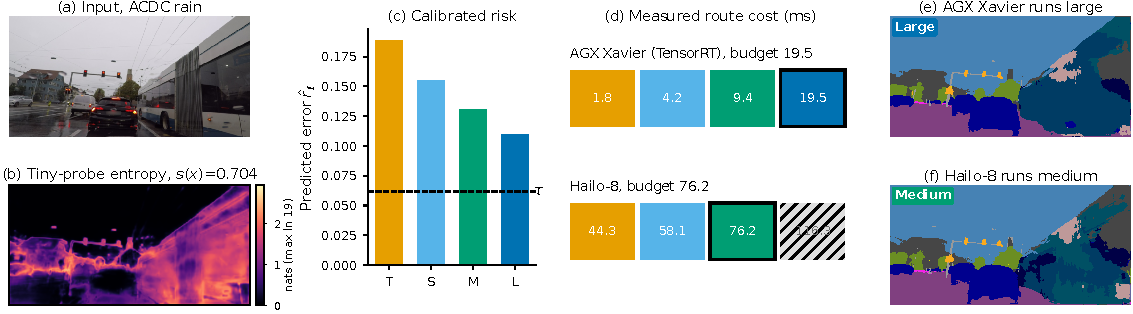
\includegraphics[width=\textwidth]{figures/fig7_routing_decision_v20.pdf}
\caption{One complete policy-D decision on a held-out ACDC rain image. (a) Input. (b) Per-pixel entropy of the tiny probe and its mean $s(x)$. (c) Candidate-specific calibrators map $s(x)$ to four predicted errors; the dashed line is the risk target $\tau$. (d) Measured median route costs on AGX Xavier and Hailo-8 under the stated budgets; infeasible routes are grey and hatched, and the selected route is outlined. (e, f) The capacity run on each device. The example illustrates the policy and is not an additional evaluation trial.}
\label{fig:input-output-pipeline}
\end{figure*}

%======================================================================
\section{Experimental setup}
\label{sec:protocol}

\subsection{Data and fit/held-out split}

Cityscapes provides 2,975 training and 500 validation images~\cite{cordts2016cityscapes}, and ACDC provides 1,600 training and 406 validation images across fog, night, rain, and snow~\cite{sakaridis2021acdc}; both use the 19 Cityscapes training classes. All models are trained on the training sets at the native 2:1 aspect ratio. Each validation split is then divided by alternating index (Table~\ref{tab:dataset-splits}): even-index images form the fit half, used for calibration and operating-point selection, and odd-index images form the held-out half, used only for evaluation. The study does not use an external test server.

\begin{table}[!t]
\centering
\caption{Dataset composition and alternating-index router split. Fit and held-out counts partition each validation subset exactly.}
\label{tab:dataset-splits}
\small
\begin{tabular}{@{}lrrrr@{}}
\toprule
Dataset/condition & Train & Validation & Fit & Held-out \\
\midrule
Cityscapes clean & 2,975 & 500 & 250 & 250 \\
ACDC fog   & 400 & 100 & 50 & 50 \\
ACDC night & 400 & 106 & 53 & 53 \\
ACDC rain  & 400 & 100 & 50 & 50 \\
ACDC snow  & 400 & 100 & 50 & 50 \\
\bottomrule
\end{tabular}
\end{table}

\subsection{Models and training runs}

Three elastic supernets are trained with seeds 0--2 (Runs A--C) under the recipe of Section~\ref{sec:elastic}, and every router experiment is repeated on all three. For RQ2, two references are trained with the same recipe and three seeds each: Fast-SCNN~\cite{poudel2019fastscnn}, and the large \method{} architecture trained alone, without weight sharing or distillation (PACE-Large). Checkpoint and configuration hashes are listed in the supplement.

\subsection{Hardware and latency measurement}

Table~\ref{tab:hardware} lists the four devices. NVIDIA devices run TensorRT FP16 engines built from the fixed-shape ONNX graphs, and Hailo-8 runs INT8 HEF files compiled from the same graphs with the Hailo Dataflow Compiler and quantized with 200 real fit-half images. All four candidates execute on both primary paths. The Jetson DLA is excluded because decoder layers fall back to the GPU, which would make the measured route a mixed-device path.

\begin{table}[!t]
\centering
\caption{Hardware and compiler stacks used for latency measurement.}
\label{tab:hardware}
\scriptsize
\begin{tabularx}{\columnwidth}{@{}l>{\raggedright\arraybackslash}p{2.1cm}>{\raggedright\arraybackslash}X@{}}
\toprule
Name & Hardware & Runtime and system versions \\
\midrule
Hailo-8 & Raspberry Pi 5 + Hailo-8 M.2 & HailoRT 4.23.0; Dataflow Compiler 3.34.0; Model Zoo 2.19.0 \\
Xavier NX & Jetson Xavier NX & L4T R35.4.1; CUDA 11.4.19; cuDNN 8.6.0.166; TensorRT 8.5.2.2 \\
AGX Xavier & Jetson AGX Xavier & L4T R35.6.4; CUDA 11.4.19; TensorRT 8.5.2.2 \\
Orin Nano & Jetson Orin Nano Super & L4T R36.5.0; CUDA 12.6.68; cuDNN 9.3.0; TensorRT 10.3.0.30 \\
\bottomrule
\end{tabularx}
\end{table}

Three kinds of latency are measured. Candidate-only latency, used for RQ1, times each candidate in isolation at batch size one on all four devices with the trtexec/hailortcli protocol; RQ1 uses the mean, and the cards of Fig.~\ref{fig:candidate-family} report p95. Complete route cost $C_h(\ell)$, used by the router, and static cost $S_h(\ell)$, used for the static references, are measured on Hailo-8 and AGX Xavier in the same process, with the same engines, inputs, and timer boundary. The timer starts when a preprocessed host tensor is handed to the runtime and stops after the returned prediction is synchronized; image decoding, resizing, and normalization are outside the timer. On AGX Xavier all four TensorRT execution contexts stay resident and the route covers tiny inference, entropy, policy evaluation, dispatch, and any additional inference. The primary Hailo-8 path uses explicit Hailo network-group activation with FLOAT32 output streams, and its route includes the activation of the selected engine; the HailoRT model scheduler and UINT8 output streams are reported as sensitivity results. Each configuration uses 50 warm-up and 500 timed iterations, with Jetson power mode recorded and temperatures logged before and after each run. Table~\ref{tab:routes} reports the medians, p95, and p99 used in replay. Cold-start costs are excluded because the two runtimes have different reload semantics.

\begin{table}[!t]
\centering
\caption{Warm complete-route cost and static cost in ms (median / p95 / p99 over 500 timed iterations, same harness). A route includes the tiny probe, risk and policy computation, dispatch or activation, and any additional candidate inference; a static deployment runs only its own engine. The median is the primary cost table; p95 and p99 tables are used for the sensitivity analysis in Section~\ref{sec:rq3}.}
\label{tab:routes}
\footnotesize
\setlength{\tabcolsep}{3pt}
\begin{tabular}{@{}lcc@{}}
\toprule
Route & AGX Xavier (TensorRT) & Hailo-8 \\
\midrule
tiny $\rightarrow$ tiny & 1.84 / 1.91 / 1.94 & 44.26 / 45.28 / 45.42 \\
tiny $\rightarrow$ small & 4.24 / 4.36 / 4.42 & 58.11 / 59.56 / 60.00 \\
tiny $\rightarrow$ medium & 9.44 / 9.78 / 9.87 & 76.18 / 78.23 / 80.16 \\
tiny $\rightarrow$ large & 19.50 / 19.59 / 19.63 & 116.26 / 118.02 / 118.93 \\
\midrule
static tiny & 1.18 / 1.21 / 1.24 & 6.27 / 6.57 / 6.61 \\
static small & 2.56 / 2.71 / 2.76 & 12.07 / 12.67 / 12.82 \\
static medium & 7.11 / 7.42 / 7.51 & 30.91 / 31.82 / 32.07 \\
static large & 16.76 / 16.92 / 17.26 & 69.39 / 70.51 / 70.98 \\
\bottomrule
\end{tabular}
\end{table}

Accuracy and latency are combined in an offline per-image replay with measured costs. Every candidate prediction is computed once per image from the trained PyTorch models and cached, and each routing decision is scored against these cached predictions while its cost is taken from the measured table. Section~\ref{sec:compiled} checks this replay against the compiled TensorRT and Hailo-8 engines with the trained weights.

\subsection{Evaluation protocol}
\label{sec:split}

Segmentation quality is dataset-level \miou{}. For a routed policy, the confusion matrices of the selected candidates are accumulated over the held-out images and \miou{} is computed once. The unit of analysis is an operating cell, defined by training run, backend cost table, split, and budget; the 120 cells reuse images and predictions and are therefore correlated, and we report descriptive win/tie/loss counts alongside bootstrap intervals.

Operating points are chosen on the fit half by a fixed rule. Five candidate risk targets $\tau$ are set to the 10th, 25th, 50th, 75th, and 90th percentiles of fit-half observed error, macro-aggregated across splits; one such grid is generated per run and shared by the two cost tables. For each budget and policy, the selected target maximizes fit-half \miou{} among targets whose mean fit-half cost meets the budget, with lower cost as the tie-break. Only then are held-out labels read, to compute routed \miou{} and budget violations. Calibrators, targets, thresholds, and operating points never see held-out labels, the entropy feature is identical at fitting and deployment, and the pooled variant combines only fit halves.

A cell is violating if at least one held-out image is routed to a candidate whose tabulated route cost exceeds the budget. This is a route-selection criterion: it guarantees that the selected route's median (or, in the sensitivity analysis, p95 or p99) cost fits the budget, not that every individual frame does. Because D removes infeasible candidates before choosing, its zero violation count is partly structural, whereas A can violate a budget whenever its threshold escalates an image to an expensive route. Comparisons with A therefore use fair cells, those in which A has no held-out violation; comparisons with A-hard and T-hard use all cells. Two budget grids are used. The \emph{route-budget grid} uses the four route costs of each device as budgets (3 runs $\times$ 2 backends $\times$ 5 splits $\times$ 4 budgets = 120 cells); every budget admits at least the tiny route, so D, A-hard, and T-hard never violate it. The \emph{static-own-cost grid} uses the union of the four route and four static costs of one device (3 runs $\times$ 5 splits $\times$ 8 budgets = 120 cells per backend). It contains budgets below the cheapest route, $C_h(\mathrm{tiny})$, which a static engine can meet but no route can, because every route starts with the probe; there D falls back to tiny and violates the budget. The primary routing-versus-static comparison therefore uses the route-feasible cells of this grid, and the all-cell result is reported only as a diagnostic. Quality differences are reported in \miou{} percentage points.

Uncertainty is estimated with an image-level bootstrap: in each of 1,000 replicates, the held-out images of every split are resampled with replacement, the same resample is applied to every run, backend, and budget of that split, routed \miou{} is recomputed, and the macro-averaged difference is recorded. We report percentile 95\% intervals; the bootstrap is paired, because both policies of a comparison are scored on the same resampled images, and it uses a fixed random seed. These intervals reflect image sampling only, not training-run variability. A nested bootstrap (200 replicates) additionally resamples the fit halves and refits calibrators, risk grid, and operating points in every replicate. Three further analyses address robustness. The cost-statistic sensitivity rebuilds both the cost table and the budget grid from the p95 or p99 costs. The leave-one-condition-out (LOCO) analysis refits the calibrators, the risk-target grid, and the operating points on the fit halves of the other four conditions only and evaluates on the held-out half of the remaining condition. Finally, a counterfactual break-even analysis scales the measured routing overhead $C_h(\ell)-S_h(\ell)$ by a factor $\alpha\in[0,1]$, keeping all predictions fixed, and repeats the comparison with static deployment; it does not measure an optimized implementation.

%======================================================================
\section{Results}
\label{sec:results}

\subsection{RQ1: Does a FLOPs-proportional proxy reproduce measured feasibility?}
\label{sec:rq1}

No. The four candidates require 0.206, 1.168, 6.171, and 22.699 GFLOPs, a $110.2\times$ range from tiny to large, but their measured mean latency grows by only $12.3$--$18.1\times$, depending on the device: $12.3\times$ on the Hailo-8 (4.0 to 49.3~ms), $17.2\times$ on AGX Xavier (1.0 to 17.2~ms), $17.5\times$ on Orin Nano (1.0 to 18.0~ms), and $18.1\times$ on Xavier NX (1.6 to 29.5~ms) (Fig.~\ref{fig:flops-latency}). The dashed lines in Fig.~\ref{fig:flops-latency} show the latency that a proxy proportional to FLOPs, anchored at each device's tiny candidate, would predict; it overestimates the cost of every larger candidate, and that of large by $6$--$9\times$ (110~ms instead of 17.2~ms on AGX Xavier, 441~ms instead of 49.3~ms on Hailo-8). The small candidates are memory- and launch-bound, so their latency falls far less than their compute, and the gap differs between devices because each accelerator handles memory traffic and small kernels differently.

\begin{figure}[!t]
\centering
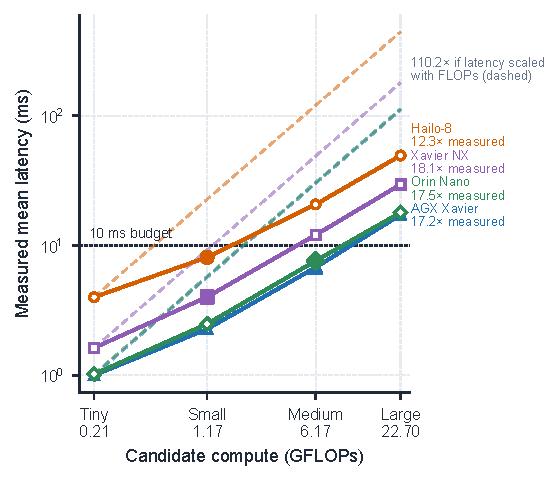
\includegraphics[width=\columnwidth]{figures/fig5_flops_latency_v20.pdf}
\caption{Measured latency versus compute. Solid lines show measured mean latency of the four candidates on each device; dashed lines in the same colour show the latency a FLOPs-proportional proxy anchored at tiny would predict. Filled markers indicate the largest candidate that fits an illustrative 10~ms budget on each device. The $110.2\times$ compute range becomes only $12.3$--$18.1\times$ measured latency.}
\label{fig:flops-latency}
\end{figure}

The mismatch changes deployment decisions. Under the illustrative 10~ms budget marked in Fig.~\ref{fig:flops-latency}, the largest feasible candidate is small on Hailo-8 and Xavier NX and medium on AGX Xavier and Orin Nano, whereas the proxy would rule out medium on AGX Xavier and Orin Nano and small on Hailo-8, all of which measurement shows to fit. Measuring the four routes once per device removes this error at negligible engineering cost. The result concerns a proportional proxy only; learned latency predictors may do better and are not evaluated here.

Isolated candidate latency is itself insufficient, because a deployed route also includes the probe and dispatch. On AGX Xavier the tiny route grows from 1.03~ms candidate-only p95 to a 1.84~ms complete-route median, and on Hailo-8 from 4.01~ms to 44.26~ms, because in the primary Hailo-8 configuration the route also includes per-call network-group activation and host-side entropy, which static deployment does not; these components were not timed separately. On Hailo-8 this expansion falls from $11.0\times$ for tiny to $2.4\times$ for large as candidate inference begins to dominate, whereas on AGX Xavier it stays between $1.1\times$ and $1.9\times$. A budget defined from candidate-only latency would admit routes that are infeasible in deployment, particularly on Hailo-8. This is why the router uses complete route costs (Table~\ref{tab:routes}).

\subsection{RQ2: Does shared elastic training preserve quality?}

Only partly. Figure~\ref{fig:rq2} compares the largest elastic capacity with the same architecture trained alone (PACE-Large) and with Fast-SCNN, each over three seeds. Shared training costs the large capacity 0.9 \miou{} points on Cityscapes ($59.0\pm0.3$ versus $60.0\pm0.5$) and 1.6--2.8 points on the ACDC conditions, 2.0 points on the ACDC mean ($49.8$ versus $51.8$); the gap is largest at night ($-2.8$). Against Fast-SCNN, the elastic large capacity is 0.8 points better on Cityscapes and 0.8--1.8 points worse on night, snow, and fog, but 4.0 points worse on rain. Our study plan had set a practical band of 1.5 points relative to an independently trained model of similar size. Against Fast-SCNN, the elastic large capacity stays within this band on Cityscapes, night, and snow but not on fog or rain; against the same architecture trained alone (PACE-Large), it stays within the band only on Cityscapes and exceeds it on all four ACDC conditions. In exchange, the same weights also provide the tiny, small, and medium capacities (33.8, 40.8, and 49.3 \miou{} on Cityscapes).

\begin{figure}[!t]
\centering
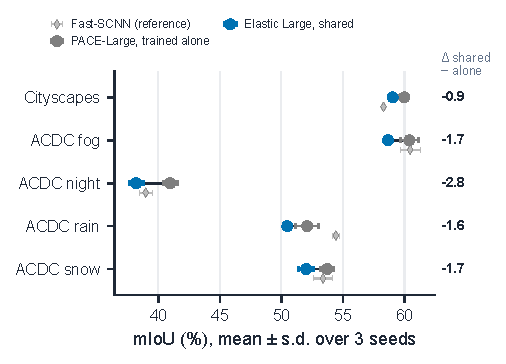
\includegraphics[width=\columnwidth]{figures/fig6_rq2_dumbbell_v20.pdf}
\caption{Weight sharing costs the largest capacity 0.9--2.8 \miou{} points. Elastic Large (shared training, blue) versus the same architecture trained alone (PACE-Large, grey) per split, mean $\pm$ s.d. over three seeds; the right column gives the difference. Fast-SCNN (diamonds) is a secondary external reference.}
\label{fig:rq2}
\end{figure}

This result matters for interpreting RQ3. A router can only choose among the candidates it is given, and the cost of weight sharing grows under adverse conditions, which is exactly where a router would most want the large capacity. All routing comparisons below are made within one supernet, so they are not affected by this gap, but a deployment that needs only the large capacity would be better served by training it alone.

\subsection{RQ3: Which routing ingredients matter, and does routing beat static deployment?}
\label{sec:rq3}

We answer RQ3 against five references: rank escalation (A), rank escalation with the same hard budget (A-hard), a three-threshold scalar router (T-hard), the best feasible static candidate, and, under mean-cost budgets, the static mixture. Table~\ref{tab:routerfinal} summarizes all comparisons in the replay with measured costs.

\begin{table*}[!t]
\centering
\caption{Routing comparisons in held-out replay with measured costs. $\Delta$: macro-averaged \miou{} difference (points); 95\% CI: paired image-level bootstrap (1{,}000 replicates, fixed seed), image sampling only; nested CI also refits calibrators, risk grid, and operating points on resampled fit halves. Cells are correlated and the two devices share predictions. (a) Route-budget grid: 3 runs $\times$ 2 backends $\times$ 5 splits $\times$ 4 budgets = 120 cells; comparisons with A use fair cells (A without violation). Violating cells (median / p95 / p99): A 58 / 58 / 59 of 120; A-hard, T-hard, D, pooled D, and LOCO D 0 of 120. ``Static, route cost'' charges the static candidate the cost of the route that ends in it. (b) Static-own-cost grid, per backend: 3 runs $\times$ 5 splits $\times$ 8 budgets = 120 cells. Primary rows use route-feasible cells; diagnostic rows use all cells and include budgets below the cheapest route, where D falls back to tiny and violates the budget (15 cells on AGX Xavier, 45 on Hailo-8). These shares are shares of the evaluated budget grid, not deadline-miss rates of a deployment.}
\label{tab:routerfinal}
\footnotesize
\setlength{\tabcolsep}{4pt}
\begin{tabular}{@{}llrrrcc@{}}
\toprule
Cost table & Comparison & Cells & W/T/L & Mean $\Delta$ & 95\% CI & Nested CI \\
\midrule
\multicolumn{7}{@{}l}{\emph{(a) Router ablation, route-budget grid}} \\
Median & D $-$ A & 62 & 54/6/2 & +2.87 & [+2.52, +3.26] & [+1.85, +3.28] \\
Median & Pooled D $-$ A & 62 & 54/6/2 & +2.90 & -- & -- \\
Median & A-hard $-$ A & 62 & 22/38/2 & +0.47 & -- & -- \\
Median & D $-$ A-hard & 120 & 48/72/0 & +1.41 & [+1.19, +1.63] & [+0.99, +1.70] \\
Median & T-hard $-$ A-hard & 120 & 46/68/6 & +1.44 & -- & -- \\
Median & D $-$ T-hard & 120 & 16/80/24 & $-0.03$ & [$-0.11$, +0.09] & -- \\
Median & D $-$ best feasible static, route cost & 120 & 0/92/28 & $-0.16$ & [$-0.22$, $-0.10$] & -- \\
p95 & D $-$ A & 62 & 54/6/2 & +2.87 & [+2.52, +3.26] & -- \\
p95 & D $-$ A-hard & 120 & 48/72/0 & +1.41 & [+1.19, +1.63] & -- \\
p99 & D $-$ A & 61 & 53/6/2 & +2.83 & -- & -- \\
Median, LOCO & D $-$ A & 41 & 29/12/0 & +4.15 & -- & -- \\
Median, LOCO & D $-$ A-hard & 120 & 48/72/0 & +1.59 & -- & -- \\
\midrule
\multicolumn{7}{@{}l}{\emph{(b) Routing versus static deployment charged its own latency, static-own-cost grid (median)}} \\
AGX Xavier & D $-$ static, route-feasible (primary) & 105 & 0/46/59 & $-3.00$ & [$-3.07$, $-2.72$] & -- \\
AGX Xavier & D $-$ static, all cells (diagnostic) & 120 & 0/61/59 & $-2.62$ & [$-2.69$, $-2.38$] & -- \\
AGX Xavier & static feasible, route infeasible & 15/120 & \multicolumn{4}{l}{12.5\% of the grid (budget 1.18~ms)} \\
Hailo-8 & D $-$ static, route-feasible (primary) & 75 & 0/6/69 & $-8.18$ & [$-8.42$, $-7.40$] & -- \\
Hailo-8 & D $-$ static, all cells (diagnostic) & 120 & 0/21/99 & $-7.41$ & [$-7.61$, $-6.76$] & -- \\
Hailo-8 & static feasible, route infeasible & 45/120 & \multicolumn{4}{l}{37.5\% of the grid (budgets 6.3, 12.1, 30.9~ms)} \\
\bottomrule
\end{tabular}
\end{table*}

\paragraph{Against rank escalation} Configured D outperforms or matches A in 60 of 62 fair cells, with a mean gain of +2.87 \miou{} points (95\% CI +2.52 to +3.26; nested +1.85 to +3.28), and it never selects a route whose tabulated cost exceeds the budget, whereas A does so in 58 of 120 cells. Pooled D, which uses one calibrator set for all conditions, records 54/6/2 and +2.90 points. Figure~\ref{fig:router-frontier} summarizes the router ablation and the static comparisons with their intervals.

\begin{figure*}[!t]
\centering
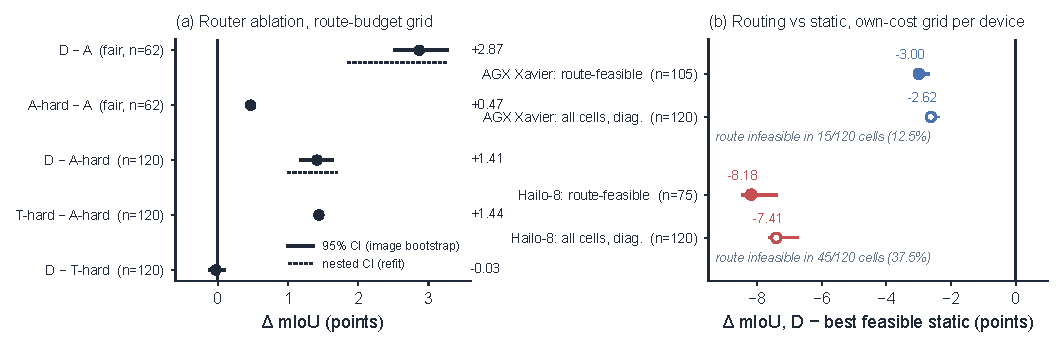
\includegraphics[width=\textwidth]{figures/fig7_two_panel_v21.pdf}
\caption{Routing gains over rank escalation come from budget-constrained operating-point tuning rather than candidate-specific calibration, and routing loses to static deployment charged its own latency. (a) Router ablation on the route-budget grid (n = 62 fair cells or 120 cells): mean \miou{} difference with paired image-level 95\% bootstrap intervals (solid) and nested intervals (dashed) where computed; rows without an interval were not bootstrapped. (b) Policy D minus the best feasible static model on each backend's static-own-cost grid: route-feasible cells (filled, primary; n = 105 and 75) and all cells including route-infeasible budgets where D violates (open, diagnostic; n = 120). Intervals reflect image sampling only, not training-seed variability.}
\label{fig:router-frontier}
\end{figure*}

\paragraph{Separating the hard budget from candidate-specific risk} D differs from A in two ways, a hard budget and candidate-specific risk. A-hard adds only the first. Adding the hard budget removes all of A's violations but improves fair-cell quality by only +0.47 points. Adding candidate-specific risk on top, which turns A-hard into D, gains a further +1.41 points (95\% CI +1.19 to +1.63; nested +0.99 to +1.70) with 48 wins, 72 ties, and no losses over all 120 cells. The same gain, however, is obtained without candidate-specific calibration: T-hard, which places three tuned thresholds directly on the entropy score, improves on A-hard by +1.44 points and differs from D by $-0.03$ points (95\% CI $-0.11$ to +0.09) at about 1\% lower cost; the interval excludes a gain of candidate-specific calibration larger than 0.09 points but does not establish formal equivalence. The advantage over rank escalation therefore comes from choosing the operating point under the hard budget on the fit half, and with a single scalar probe we detect no benefit of the four calibrators over a monotone threshold rule.

\paragraph{Robustness} Replacing the median cost table by the p95 or p99 table, for both the costs and the budget grid, leaves the conclusions unchanged: D still selects no route whose tabulated cost exceeds the budget, and its gains over A and A-hard change by at most 0.04 points. Calibrators fitted without the evaluated condition (LOCO) also keep D free of violations and ahead of A-hard by +1.59 points, so the gain does not depend on having calibrated on the test condition itself. On the held-out halves, the four candidate-specific calibrators have mean absolute errors of 0.019--0.057 in per-image pixel error, lie close to the diagonal of a reliability plot, and change by at most 0.003 when the ten equal-count bins are replaced by five bins or isotonic regression (supplement, Fig.~S2). The absence of a detectable gain of D over T-hard is therefore not explained by poor calibration.

\paragraph{Against static deployment} The comparison with static deployment depends on what the static model is charged. If it is charged the cost of the route that ends in it, as if it also paid for the probe, D stays within 0.16 points of the best feasible static candidate (95\% CI $-0.22$ to $-0.10$), tying in 92 of 120 cells and lowering the mean route cost by 2.0\%; the non-deployable GT pixel-error oracle exceeds that static reference by only 0.11 points, so the headroom for per-image routing under a per-frame cap is small with this candidate set. A static deployment, however, does not run the probe. Figure~\ref{fig:routestatic} shows the same-harness latency of each capacity deployed statically and reached through the tiny probe. On AGX Xavier a route costs 0.7~ms more than the static engine it ends in for tiny and 2.7~ms more for large; on Hailo-8 the overhead is 38--47~ms, comparable to the full latency of the large engine, and it does not shrink with the HailoRT scheduler or UINT8 output streams. Charged its own latency, static deployment is compared with routing on each backend's static-own-cost grid (Table~\ref{tab:routerfinal}b, Fig.~\ref{fig:router-frontier}b). Part of this grid lies below the cheapest route: because every route begins with the tiny probe, budgets below $C_h(\mathrm{tiny})$ can be met by the static tiny engine but by no route. This holds for 15 of 120 cells on AGX Xavier (12.5\%) and 45 of 120 cells on Hailo-8 (37.5\%); in these cells D falls back to tiny and violates the budget. On the route-feasible cells, the primary comparison, the best feasible static model beats D by 3.00 points on AGX Xavier (95\% CI $-3.07$ to $-2.72$; 0 wins, 46 ties, 59 losses over 105 cells) and by 8.18 points on Hailo-8 with FLOAT32 output streams ($-8.42$ to $-7.40$; 0/6/69 over 75 cells), and by 10.97 points with UINT8 streams; T-hard behaves the same ($-2.99$ and $-8.17$). Including the route-infeasible cells, a diagnostic that mixes in budget-violating routing actions, gives $-2.62$ and $-7.41$ points. The two subsets differ in their budgets, so the larger deficit on feasible cells should not be read as stronger evidence; both show that static deployment is better.

\begin{figure*}[!t]
\centering
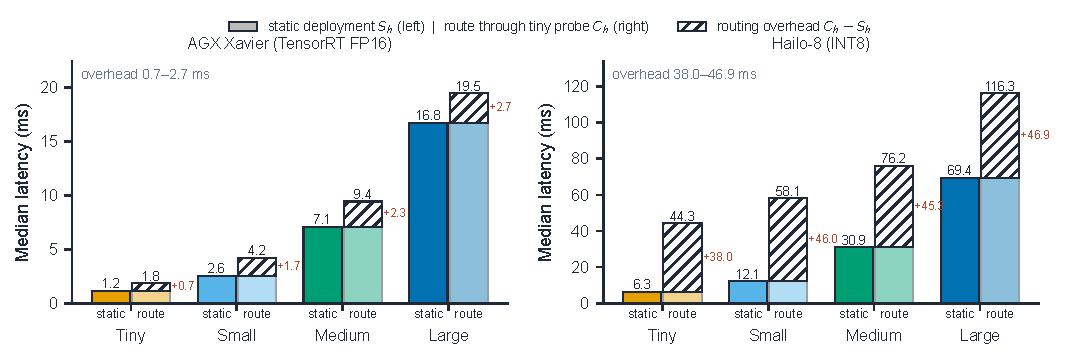
\includegraphics[width=\textwidth]{figures/fig11_route_vs_static_v20.pdf}
\caption{The routing overhead is small on the TensorRT GPU but comparable to a full large-model inference on the Hailo-8. Same-harness median latency of each capacity deployed statically ($S_h$, left bars) and reached through the tiny probe ($C_h$, right bars); the hatched segment is the overhead $C_h-S_h$, labelled in ms. AGX Xavier returns logits; Hailo-8 uses explicit network-group activation with FLOAT32 output streams.}
\label{fig:routestatic}
\end{figure*}

\paragraph{Mean-cost budgets and break-even overhead} When only the average cost is constrained, the fairer static reference is a random mixture of the two adjacent static models with the same mean cost. Charged their own latencies, candidate-specific routing still loses to this mixture by 0.3--0.5 points on AGX Xavier and 5.5--6.3 points on Hailo-8. To ask how much the overhead would have to shrink, we scale the measured per-capacity overhead by $\alpha\in[0,1]$ in a counterfactual replay, with predictions held fixed, and repeat the comparison (Fig.~\ref{fig:breakeven}). With zero overhead, routing would gain 1.3--1.4 points over static mixing on both devices; the gain vanishes at 1.3~ms of overhead on AGX Xavier (measured: 1.9~ms) and 4.3~ms on Hailo-8 (measured: 44~ms). These break-even values describe how small the overhead would need to be; no implementation with such overhead was measured. Under per-frame budgets routing never wins, even at zero overhead ($-0.16$ points), because any per-frame cap forces the router to stay at or below the capacity that the static model already uses.

\begin{figure*}[!t]
\centering
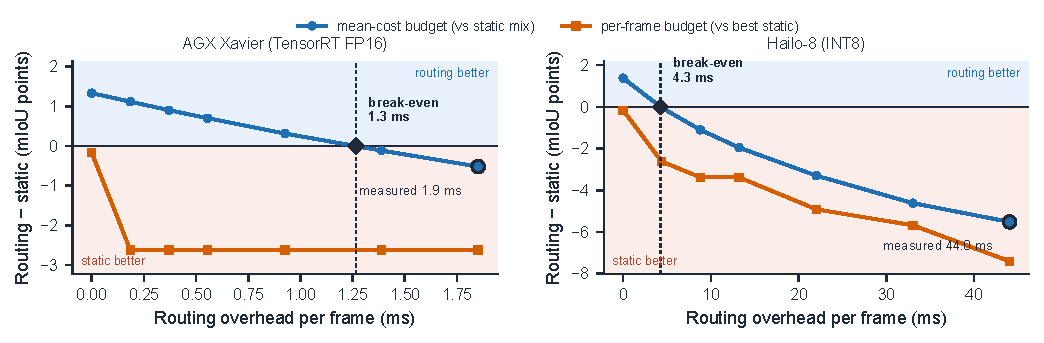
\includegraphics[width=\textwidth]{figures/fig12_breakeven_v20.pdf}
\caption{Counterfactual overhead scaling: routing would pay off only under mean-cost budgets and only below a small break-even overhead. Routing minus static \miou{} as the measured routing overhead is scaled from zero to its measured value (circle), with predictions held fixed; shading marks where routing (blue) or static deployment (red) is better. Blue line: mean-cost budgets against static mixing; orange line: per-frame budgets against the best feasible static model, which stays below zero at every overhead. Diamonds: break-even overhead.}
\label{fig:breakeven}
\end{figure*}

Table~\ref{tab:router-condition} breaks the comparison with A down by condition, with 24 cells per row from three runs and two cost tables. The gain over A is largest on clean Cityscapes (+8.81 points), although only 6 of its 24 cells are fair because A violates the budget in the other 18. Rain is the opposite case: A violates a budget in only 3 cells, and configured D records 15 wins, 6 ties, and no losses over 21 fair cells with a +2.09-point gain. Night has the smallest gain, +1.05 points, despite winning all 14 fair cells. The only two losses occur on snow, for both configured and pooled D. No single condition drives the aggregate result, and fair-cell counts and violation counts must be read together.

\begin{table}[!t]
\centering
\caption{Condition-level comparison against policy A (median cost tables). W/T/L and mean $\Delta$ use fair cells; violation counts use all 24 cells per condition. Configured and pooled D each have zero violations.}
\label{tab:router-condition}
\scriptsize
\setlength{\tabcolsep}{2.0pt}
\resizebox{\columnwidth}{!}{%
\begin{tabular}{@{}lrrrrrrr@{}}
\toprule
Condition & Fair & Config. W/T/L & Config. $\Delta$ & Pooled W/T/L & Pooled $\Delta$ & A viol. & D viol. \\
\midrule
Cityscapes & 6/24 & 6/0/0 & +8.81 & 6/0/0 & +8.87 & 18/24 & 0/24 \\
ACDC/Fog & 9/24 & 9/0/0 & +5.38 & 9/0/0 & +5.51 & 15/24 & 0/24 \\
ACDC/Night & 14/24 & 14/0/0 & +1.05 & 14/0/0 & +1.08 & 10/24 & 0/24 \\
ACDC/Rain & 21/24 & 15/6/0 & +2.09 & 15/6/0 & +2.11 & 3/24 & 0/24 \\
ACDC/Snow & 12/24 & 10/0/2 & +1.49 & 10/0/2 & +1.48 & 12/24 & 0/24 \\
\bottomrule
\end{tabular}
%
}
\end{table}

The small night gain is consistent with the probe. The large candidate reaches 59.0 \miou{} on Cityscapes but only 38.2 on ACDC night, and the night calibrators have the largest held-out errors (0.051--0.057) and the weakest score--error rank correlation (Spearman 0.35--0.67, against 0.74--0.81 on Cityscapes). The entropy score thus ranks errors least reliably exactly where errors are most frequent. Figure~\ref{fig:qualitative} shows one representative held-out image per capacity that policy D selects.

\begin{figure*}[!t]
\centering
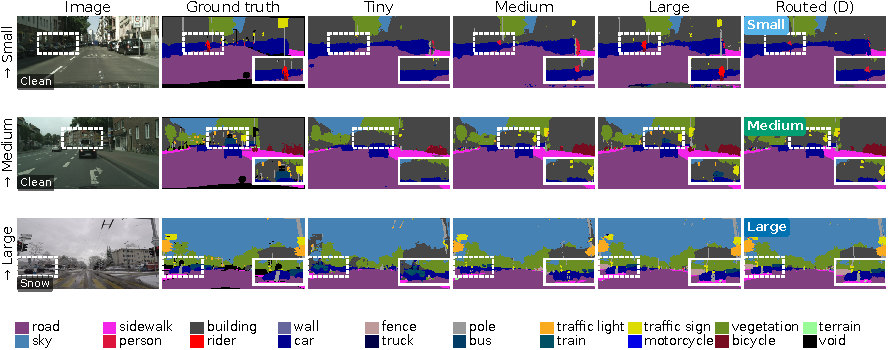
\includegraphics[width=\textwidth]{figures/fig10_stratified_v20.pdf}
\caption{Input adaptivity on held-out images. Selection rule fixed before inspection: policy D of Run A on AGX Xavier at the budget of the large route, pooled over the five held-out splits; for each capacity that D selects, the image whose selected-capacity pixel error is closest to the median of that route class. D selected tiny for none of the 453 images at this budget, small for 27, medium for 61, and large for 365. Columns show the input, ground truth (void in black), the tiny, medium, and large candidates, and the routed output with its selected capacity. Dashed boxes mark the window where tiny and large disagree most; the inset at the bottom right of each panel enlarges it.}
\label{fig:qualitative}
\end{figure*}

\subsection{Compiled-engine accuracy and on-device replay}
\label{sec:compiled}

The replay above uses PyTorch predictions. Compiled TensorRT FP16 engines with the trained weights reproduce PyTorch within $\pm0.02$ points on every capacity and split, with 99.7--100\% pixel agreement and a probe-entropy error below $2\times10^{-4}$. Hailo-8 INT8 engines lose up to 1.6 points on tiny (pixel agreement down to 87\% at night) and at most 0.5 points on large; the probe entropy deviates by 0.012--0.035 on average but keeps a rank correlation of at least 0.88. Replaying Run A with the on-device predictions and probe scores leaves every conclusion unchanged: on AGX Xavier D differs from the PyTorch replay by 0.01 points, and on Hailo-8 D loses a further 0.6 points but still matches T-hard ($-0.06$) and trails static deployment by 7.9 points.

%======================================================================
\section{Discussion}
\label{sec:discussion}

\subsection{When adaptive routing pays off}

The comparison with static deployment is the central result. Routing can only pay off if choosing per image is worth more than its cost. The headroom is small: the GT pixel-error oracle exceeds the best feasible static candidate by only 0.11 points under a per-frame cap, and even at zero overhead routing gains only 1.3--1.4 points over static mixing under a mean-cost budget. Against that, every route pays for the tiny engine, the entropy and decision, and on the Hailo-8 a per-call network-group activation; the share of each component was not measured. Routing therefore becomes worthwhile only when three conditions hold: the budget constrains mean rather than per-frame cost; the overhead stays below the counterfactual break-even value (about 1.3~ms on AGX Xavier and 4.3~ms on Hailo-8 here); and the candidates differ enough per image to leave headroom. For a fixed per-frame budget, a static model of the largest feasible capacity is the stronger choice and should always be reported as a baseline, timed in the same harness as the adaptive pipeline; at budgets below the cheapest route, only the static model can comply.

\subsection{What drives the gain among routers}

Policies A and D read the same probe score, yet they diverge at tight budgets. A maps the score to a latency rank and escalates whenever the score crosses its threshold; nothing in that rule prevents escalation to a route whose measured cost exceeds the budget, so A's operating point must be chosen conservatively, or it violates the budget, as it does in 18 of 24 Cityscapes cells. Imposing the budget alone repairs the violations but improves fair-cell quality by only +0.47 points, whereas the remaining +1.41 points come from choosing, within the feasible set, an operating point tuned on the fit half. T-hard obtains a gain of the same size with three thresholds on the raw score; with one scalar probe we detect no benefit of the four candidate-specific calibrators, which remain an interpretable way to make that choice. A richer probe, for example per-class or spatial uncertainty, would be needed for candidate-specific calibration to carry information that a threshold rule cannot.

\subsection{Deployment guidance}

For a new accelerator, the results suggest a simple procedure: compile the fixed candidate set, measure complete routes and static deployments with the production runtime in the same harness, preferably reporting tail percentiles as well as the median, and compare the routing overhead with the break-even value before deploying a router. Designs that reuse the probe computation inside the selected candidate, keep all candidates resident without switching (multi-context compilation on Hailo, one engine with shared early layers on TensorRT), or route among models with more complementary errors attack exactly the terms that make routing lose here. If a router is used, pooled calibration produced the same result as configured calibration (54/6/2 against A) and, in the LOCO analysis, transferred to a condition it had not seen, so it is the simpler default; a threshold router is simpler still. Because the probe is the tiny candidate, its quality bounds the information available to the router; the smallest gains occurred at night, where the probe ranks errors worst.

\subsection{Relation to latency predictors and dynamic networks}

The study does not compare against learned latency predictors~\cite{zhang2021nnmeter}, and RQ1 is not evidence against them. With four candidates, measuring every route is cheap and exact; with a large search space such as Once-for-All~\cite{cai2020ofa}, measurement becomes impractical and a predictor is needed, at the cost of predictor error in the feasibility test. Likewise, \method{} gives up the fine granularity of in-graph dynamic networks for compatibility with static compilers. In-graph methods avoid the engine switch that is part of the Hailo-8 route overhead, but they also need an accelerator that supports data-dependent control flow; whether a larger static candidate set would increase per-image headroom without weakening calibration remains open.

\subsection{Limitations and threats to validity}
\label{sec:limitations}

\emph{Data.} Calibration is evaluated on Cityscapes and four ACDC conditions. The LOCO analysis withholds one condition at a time, but all five conditions come from the same two datasets and camera setups, so transfer to new sensors or cities is untested. The fit and held-out halves alternate by image index rather than by sequence or location, so correlated neighbouring frames may fall on both sides; the alternating halves are not an external test set. Fit halves of 50--250 images per split leave about five images per calibration bin on the smaller ACDC splits, although five bins and isotonic regression gave nearly identical held-out errors. The calibration target is per-image pixel error, which agrees only moderately with per-image $1-$\miou{} (Spearman 0.23--0.58 across splits); routing on a class-balanced target may favour rare classes more.

\emph{Statistics.} The 120 operating cells reuse images, predictions, and thresholds and are not independent samples. The image-level bootstrap intervals capture image sampling variation but not training-run variation; the nested bootstrap adds fit-half resampling, and three seeds per model are too few to estimate seed variance precisely.

\emph{Measurement.} Accuracy under routing is replayed offline from recorded predictions with measured costs rather than in a closed-loop deployment, and compiled-engine accuracy and the on-device replay cover one of the three supernets. The zero-violation result holds on the route-budget grid and is a route-selection property with respect to tabulated median, p95, or p99 costs, not a measured per-frame deadline guarantee; it is partly structural, and it does not extend to budgets below the cheapest route, where no route can comply. The Hailo-8 route overhead was measured as a total; its components were not timed separately.

\emph{Scope.} The study has four candidates, one entropy probe, two complete-route backends, and no energy measurement. Cold-start behaviour, temporal routing across video frames, and class-level error analysis are left to future work.

%======================================================================
\section{Conclusion}
\label{sec:conclusion}

We measured when input-adaptive semantic segmentation pays off on edge accelerators. On four edge devices, a FLOPs-proportional proxy did not reproduce measured budget choices, so feasibility should come from measured complete inference routes. Shared elastic training cost the largest capacity 0.9 \miou{} points on Cityscapes and 1.6--2.8 points on ACDC relative to training it alone. Among routers, a hard measured budget with fit-half operating-point tuning is what matters: it lifted routing 2.87 points over rank escalation, its selected routes fit the tabulated median, p95, and p99 costs on the route-budget grid, and candidate-specific calibration showed no detectable gain over a three-threshold scalar router. Charged its own measured latency, however, static deployment beat routing on both a TensorRT GPU and a Hailo-8 by 3.0 and 8.2 points at route-feasible budgets, and only static deployment could meet the lowest budgets; in a counterfactual analysis, routing would break even under mean-cost budgets only if its overhead fell below about 1.3 and 4.3~ms. Adaptive-inference studies on edge hardware should therefore report a static baseline timed in the same harness and the break-even overhead of their routing pipeline. Offline replay, an index-based split, and the absence of energy measurement bound these claims.

\section*{CRediT authorship contribution statement}

% TODO(author): adjust roles if co-authors are added.
\textbf{D\~ung Nguy\~{\^e}n:} Conceptualization, Methodology, Software, Validation, Formal analysis, Investigation, Data curation, Visualization, Writing -- original draft, Writing -- review \& editing.

\section*{Declaration of competing interest}

% TODO(author): confirm. Replace with a disclosure if any financial or personal relationship could be perceived as influencing this work.
The authors declare that they have no known competing financial interests or personal relationships that could have appeared to influence the work reported in this paper.

\section*{Funding}

% TODO(author): replace with funder names and grant numbers, or keep the standard no-funding sentence.
[FUNDING STATEMENT TO BE PROVIDED.]

\section*{Data availability}

The implementation, experiment reports, canonical result artifacts, and a separate supplement containing detailed provenance, runtime versions, and extended qualitative and routing analyses are recorded in the project repository [REPOSITORY URL OR DOI]. Cityscapes and ACDC are publicly available from their providers and are subject to their respective licenses; they are not redistributed.

\section*{Acknowledgements}

% TODO(author): add individuals who helped with the research, or remove this section.
[ACKNOWLEDGEMENTS TO BE PROVIDED.]

\section*{Declaration of generative AI and AI-assisted technologies in the manuscript preparation process}

During the preparation of this work the author used Claude (Anthropic) in order to assist with language editing, manuscript structuring, LaTeX formatting, analysis scripts, and scripts that render figures from the recorded experimental results. After using this tool, the author reviewed and edited the content as needed and takes full responsibility for the content of the published article.

\bibliographystyle{elsarticle-num}
\bibliography{references}

\end{document}
